\section{Desarrollo}

\subsection{Inducción matemática}

Inducción matemática es una técnica utilizada para probar declaraciones o proposiciones.
La idea es similar a la de hacer caer varias piezas de dominó.
\begin{figure}[htb]
    \centering
    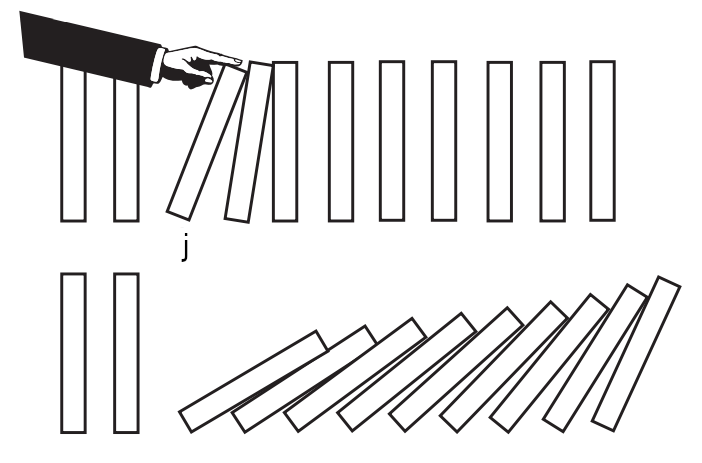
\includegraphics[width=7cm]{images/dominoes-fall}
    \caption{Fichas de dominó cayendo.}
    \label{fig:figure}
\end{figure}
Si cada pieza está lo suficientemente cerca de la anterior y hacemos caer la primera, entonces todas las piezas eventualmente van a caer.
Cuando queremos demostrar que una proposición se cumple sobre números naturales, la idea es la misma.
Dicho de otro modo, la inducción nos permite demostrar una propiedad en \textbf{infinitos números} con \textbf{pasos finitos}.

\begin{principle.box}{Inducción simple}{}
    Sea el entero $j$ y $S(n)$ una proposición sobre el entero $n$ con $n \geq j$,
    \begin{itemize}
        \item[i)] si $S(j)$ es cierto, y
        \item[ii)] para cada entero $k \geq j$, $S(k) \implies S(k + 1)$,
    \end{itemize}
    entonces $S(n)$ es cierta para todo $n \geq j$.
\end{principle.box}

Asi por ejemplo, si tenemos $j = 1$ y una proposición $S(n)$ cumple las dos condiciones anteriores, entonces $S(n)$
se cumple (es cierta) para todo natural $n$.


\begin{principle.box}{Inducción fuerte}{}
    Sea el entero $j$ y $S(n)$ una proposición sobre el entero $n$ con $n \geq j$,
    \begin{itemize}
        \item[i)] si $S(j)$ es cierto para todo $j \geq i$, y
        \item[ii)] para cada entero $k \geq j$, $S(j), S(j+1), \ldots, S(k - 1), S(k) \implies S(k + 1)$,
    \end{itemize}
    entonces $S(n)$ es cierta para todo $n \geq j$.
\end{principle.box}



\subsection{Descenso infinito de Fermat}

Sigamos con otro principio, uno bastante intuitivo.
\begin{principle.box}{Buen orden}{}
    Para todo subconjunto no vacío de los naturales, este debe tener un elemento mínimo.
\end{principle.box}
De igual manera, es fácil pensar que un subconjunto no vacío de los números naturales debe tener un elemento máximo,
por consiguiente, cualquier subconjunto no vacío debe tener un elemento mínimo y máximo.
Al trata de problemas en específicos, a menudo utilizamos estas nociones del principio de Buen orden, lo cual podemos
formalizar con el siguiente axioma.

\begin{axiom}[Axioma del Orden]
    Si $M$ es un conjunto de $n$ números reales distintos, entonces podemos escribirlo como $M = \{x_1,x_2,\ldots,x_n\}$
    con $x_1 < x_2 < \ldots < x_n$.
\end{axiom}

El descenso infinito proviene de resolver ecuaciones diofánticas indeterminadas, el matemático Pierre de Fermat
(1601-1665) utilizó este método hace unos 400 años cuando demostró que no existe una solución entera positiva
para\footnote{Se recomienda al lector buscar la solución de Fermat, para enrriquecer su lectura.} $x^4 + y^4 = z^4$.

\begin{principle.box}{Descenso infinito de Fermat}{}
    Sea el entero no negativo $k$ y $S(n)$ una proposición sobre $n$,
    \begin{enumerate}
        \item[i)] si $S(k)$ no es cierto, y
        \item[ii)] para un $m > k$ con $S(m)$ cierto, implica un $m > r > k$ con $S(r)$ cierto,
    \end{enumerate}
    entonces $S(n)$ no es cierto para toda $n\geq k$.
\end{principle.box}
Podemos ver el DIF metafóricamente con una escalera con las siguientes propiedades; si un escalón más alto no se puede
alcanzar sin primero alcanzar un escalón más bajo, y no existe un escalón más bajo
en la escalera, entonces es imposible alcanzar algún escalón.

Veamos dos variantes o casos concretos de este principio, útiles en el estudio de las ecuaciones diofánticas.
\begin{enumerate}
    \item[i)] No existe una secuencia $n_1 > n_2 > n_3 > \ldots$ estrictamente decreciente de enteros no negativos.
    \item[ii)] Si se tiene la secuencia $n_1\geq n_2 \geq n_3 \geq \ldots$ de enteros no negativos, entonces existe un $k \geq 1$ tal que $n_k = n_{k+1} = n_{k + 2} = \cdots$.
\end{enumerate}

Cabe destacar que los principios de Inducción matemática, Buen orden y Descenso infinito son de hecho equivalentes en
el conjunto de los enteros no negativos ($\Z^{\geq 0}$).
Con lo cual, si tomamos uno es posible demostrar con este los dos restantes\footnote{Se recomienda al lector investigar cómo son esas demostraciones}.

\begin{example}
    Probar que la ecuación $x^2 + y^2 = 3z^2$ no tiene soluciones $(x,y,z)$ en enteros positivos cuando $z \neq 0$.
\end{example}
\begin{solution}
    Supongamos que hay al menos una solución $(x_1,y_1,z_1)$ con $z_1 > 0$, es claro que en módulo 3 llegamos a $x_1^2+y_1^2 \modulo{0}{3}$.
    Como los cuadrados perfectos solo dejan resto $0$ o $1$ en módulo tres, necesariamente $x_1^2\equiv y_1^2 \modulo{0}{3}$,
    por lo cual $x_1 = 3x_2$, $y_1 = 3y_2$ con $x_1 > x_2$ y $y_1 > y_2$.

    Al reemplazar en la ecuación $9x_2^2+9y_2^2=3z_1^2 \iff 3(x_2^2+y_2^2)=z_1^2 \iff 3 \mid z_1^2 \iff 3 \mid z_1$.
    Si tomamos $z_1 = 3z_2$ con $z_1 > z_2$, entonces
    \[
        x_2^2+y_2^2=3z_2^2.
    \]
    Es decir, hemos encontrado una ecuación idéntica a la original con solución $(x_2,y_2,z_2)$.
    Al analizar esta solución, obtendríamos una nueva solución $(x_3,y_3,z_3)$, de la misma manera, aplicando este proceso
    obtendríamos soluciones $(x_4,y_4,z_4)$, $(x_5,y_5,z_5)$, $(x_6,y_6,z_6)$ y así sucesivamente.
    Sin embargo, esto implica que
    \begin{align*}
        x_1 > x_2 > x_3 > \cdots, &&
        y_1 > y_2 > y_3 > \cdots, &&
        z_1 > z_2 > z_3 > \cdots
    \end{align*}
    Lo cual no es posible, luego la ecuación original no tiene soluciones.
\end{solution}




\subsection{Ejercicios y problemas}

Ejercicios y problemas para el autoestudio.

\begin{exercise}
    Hallar las soluciones enteras no negativas $(x,y,z)$ tal que $x^3 + 2y^3 = 4z^3$.
\end{exercise}

\begin{problem}
    Hallar todos los enteros $a,b \in \nonnegativeSet{\Z}$ tales que $a^2 + b^2 + c^2 = a^2 b^2$.
\end{problem}




\begin{exercise}
    Probar que no existen números racionales $x,y,z$ que satisfacen
    \[
        x^2+ y^2 + z^2 + 3(x+y+z) + 5 = 0.
    \]
\end{exercise}



\begin{problem}
    Encuentre todas las soluciones enteras de la ecuación $a^2-2b^2=0$.
\end{problem}

\begin{problem}
    Encuentre todas las soluciones $(x,y,z)$  enteras de las siguiente ecuación $2005x^3=y^3+25z^3$.
\end{problem}

\begin{problem}
    Resolver en los enteros no negativos la ecuación $x^3+2y^3=4z^3$.
\end{problem}

\begin{problem}
    Muestre que no hay enteros positivos $x,y,z$ tales que $x^2+10y^2=z^2$.
\end{problem}

\begin{problem}
    Encuentre todas las tripletas $(x,y,z)$ de soluciones enteras positivas a la ecuación $x^3 + 3y^3 + 9z^3 - 3xyz = 0$.
\end{problem}

\begin{problem}
    Encuentre todos los enteros $x,y,z$ tales que $x^2+y^2+z^2-2xyz=0$.
\end{problem}


\begin{problem}
    Probar que $\forall n \in \N$, la ecuación $x^2+y^2 = z^n$ tiene soluciones enteras.
\end{problem}

\begin{problem}
    Probar que $\forall n \in \N$, la ecuación $x^2+xy+y^2 = 7^n$ tiene soluciones enteras.
\end{problem}

\begin{problem}
    Probar que $\forall n \in \N$, la ecuación $(x^2 + y^2)(u^2 + v^2 + w^2) = 2009^n$ tiene soluciones enteras.
\end{problem}

\begin{problem}
    Resuelva la ecuación con enteros positivos distintos
    \[
        x_1^2 + x_2^2 + \dots + x_{2002}^2 = 1335\left(x_1 + x_2 + \dots + x_{2002}\right).
    \]
\end{problem}